\documentclass[notheorems]{beamer}
\usepackage{SlideStyle}
\renewcommand{\d}{\operatorname{d}}

\titlegraphic{\vspace*{-7cm}
    \parbox[c]{3cm}{
\includegraphics[height=.7cm]{bsulogo}}
    \hspace*{1cm}%
    \parbox[c]{2cm}{
\includegraphics[height=0.6cm]{FPMIlogo_new}}
    \hspace*{1cm}%
    \vspace*{3cm}
}

\title[Модели распространения заболеваний]{\Large CТАТИСТИЧЕСКИЙ АНАЛИЗ РАСПРОСТРАНЕНИЯ ЗАБОЛЕВАНИЙ}


\author[В. А. Гут]{Гут Валерия Александровна}

\institute[]{Научный руководитель: С.В. Лобач}


\date[]{}%{\scriptsize \structure{2017-2018}}


\begin{document}

\begin{frame}[plain]
  \titlepage
\end{frame}


%--------------------------------------------------------------------------------------
\begin{frame}{Цели и задачи работы}

1. Рассмотрение различных математических моделей по распознаванию  заболеваний

2. Получение основного дифференциального уравнения базовой модели SIR, получение приблизительных аналитического и численного решений. Исследование модификаций базовой модели SIR.

3. Исследование расширений базовой модели SIR.

4. Моделирование распространения гриппа на основе моделей SEIR.


\end{frame}

%--------------------------------------------------------------------------

\begin{frame}
	{Математические модели распространения заболеваний}
	\begin{itemize}
		\item классическая модель SI (Susceptible-Infectious);
		\item базовая модель SIR (Susceptible-Infectious-Recovered);
		\item SIS
		\item SIRD
		\item SIRS
		\item с учетом рождаемости и смертности особей
		\item SEIR
		\item MSIR
		\item MSEIR
	\end{itemize}
\end{frame}

%--------------------------------------------------------------------------

\begin{frame}
	\frametitle{Модель SI}
	Классическая модель SI разбивает предполагает, что все население делится на две группы:
	\begin{itemize}
		\item $S(t)$ = \{люди, подверженные заболеванию (susceptible) в момент времени $t$\};
		\item $I(t)$ = \{инфицированные люди (infectious) в момент времени $t$\}.
	\end{itemize}
	Введем также обозначение $N = \operatorname{const}$ --- общая численность населения.
	
	Ввиду этих обозначений имеет место запись $S(t) + I(t) = N.$
	Скорость изменения числа здоровых и больных людей задается системой ОДУ 
	\begin{eqnarray}
		\left\{ 
		\begin{gathered} 
			\begin{aligned}
				\dfrac{\d S(t)}{\d t} = -\beta\cdot S(t)\cdot I(t),\\
				\dfrac{\d I(t)}{\d t} = \beta\cdot S(t)\cdot I(t),
			\end{aligned}
		\end{gathered} 
		\right.
	\end{eqnarray}
	где $\beta$ -- вероятность заражения здорового человека при контакте с больным.
\end{frame}

%--------------------------------------------------------------------------

\begin{frame}
	\frametitle{Базовая модель SIR}
	Модель SIR основана на разделении населения на три группы: 
	\begin{itemize}
	\item $S(t)$ = \{люди, подверженные заболеванию (susceptible) в момент времени $t$\};
	\item $I(t)$ = \{инфицированные люди (infectious) в момент времени $t$\};
	\item $R(t)$ = \{люди, имеющие иммунитет к болезни (recovered)\}.
	\end{itemize}
	Тогда $S + I + R = N,$ где $N=\operatorname{const}$ -- общая численность населения.
	Модель SIR задается в общем виде системой ОДУ 
	\begin{equation}
		\left\{ 
		\begin{gathered} 
			\begin{aligned}
				\dfrac {\d S(t)}{\d t} &= -\beta \cdot S(t) \cdot I(t),\\
				\dfrac{\d I(t)}{\d t} &= \beta \cdot S(t)\cdot I(t) - \gamma\cdot I(t),\\
				\dfrac{\d R(t)}{\d t} &= \gamma\cdot I(t),
			\end{aligned}
		\end{gathered} 
		\right.
	\end{equation}
	где $\gamma$ -- интенсивность выздоровления.
\end{frame}

%--------------------------------------------------------------------------

\begin{frame}{Модель SIRS}
	 Модель SIRS (Susceptible-Infected-Recovered-Susceptible) является вариацией модели SIR, которая учитывает возможность повторного заражения после выздоровления (потери иммунитета). В модели SIRS существует циклическое движение между состояниями подверженных ($S$), инфицированных ($I$) и восстановленных ($R$). Эта модель задается системой обыкновенных дифференциальных уравнений
	\begin{equation}
		\left\{ 
		\begin{gathered} 
			\begin{aligned}
				\dfrac {\d S(t)}{\d t} &= -\beta \cdot S(t) \cdot I(t) + \lambda \cdot R(t),\\
				\dfrac{\d I(t)}{\d t} &= \beta \cdot S(t)\cdot I(t) - \gamma\cdot I(t),\\
				\dfrac{\d R(t)}{\d t} &= \gamma\cdot I(t) - \lambda \cdot R(t),
			\end{aligned}
		\end{gathered} 
		\right.
	\end{equation}
	где число $\lambda$ определяет вероятность потери иммунитета и перехода из группы $R(t)$ в группу $I(t)$.
\end{frame}

%--------------------------------------------------------------------------

\begin{frame}
	{SEIR-модель}
	В SEIR модели предполагается, что инфекция имеет инкубационный (exposed) период, в течение которого люди инфицированы, но
	еще не заразны. Эта группа людей обозначается через $E(t)$. С учетом нового класса получаем следующую структуру
	популяции:
	$S + E + I + R = N = \operatorname{const}.$
	
	Модель SEIR задается в общем виде системой ОДУ
	\begin{equation}
		\left\{ 
		\begin{gathered} 
			\begin{aligned}
				\dfrac {\d S(t)}{\d t} &= - \beta \cdot I(t)\cdot S(t),\\
				\dfrac {\d E(t)}{\d t} &= \beta \cdot S(t)\cdot I(t) - \sigma\cdot E(t),\\
				\dfrac{\d I(t)}{\d t} &=\sigma \cdot E(t) - \gamma\cdot I(t),\\
				\dfrac{\d R(t)}{\d t} &= \gamma\cdot I(t). 
			\end{aligned}
		\end{gathered} 
		\right.
	\end{equation}
	параметр $\sigma^{-1}$ представляет собой среднюю продолжительность инкубационного периода.
\end{frame}

%--------------------------------------------------------------------------

\begin{frame}
	{Модели SIR с учетом смертности и рождаемости}
	Пусть $\lambda > 0$ и $\mu > 0$ коэффициенты рождаемости и смертности популяции соответственно. Система ОДУ для SIR-модели в предположении, что все рожденные являются здоровыми людьми, имеет вид 
	\begin{equation}
		\left\{ 
		\begin{gathered} 
			\begin{aligned}
				\dfrac {\d S(t)}{\d t} &= -\beta \cdot S(t) \cdot I(t) + \lambda\cdot N(t) - \mu\cdot S(t),\\
				\dfrac{\d I(t)}{\d t} &= \beta \cdot S(t)\cdot I(t) - \gamma\cdot I(t) - \mu\cdot I(t),\\
				\dfrac{\d R(t)}{\d t} &= \gamma\cdot I(t) - \mu \cdot R(t),
			\end{aligned}
		\end{gathered} 
		\right.
	\end{equation}
	где $S(t) + I(t) + R(t) = N(t).$
	
	Складывая все уравнения системы, мы получаем уравнение Мальтуса для численности популяции 
	\begin{equation}
		\dfrac{\d N(t)}{\d t} = (\lambda-\mu) \cdot N(t).
	\end{equation}
\end{frame}

%--------------------------------------------------------------------------

\begin{frame}{Модель MSIR}
		Модель MSIR (M -- «maternally derived immunity») включает класс $M(t)$ (для материнского иммунитета) в начало модели. Модель MSIR с учетом смертности и рождаемости описывается следующими дифференциальными уравнениями:
	\begin{equation}
		\left\{ 
		\begin{gathered} 
			\begin{aligned}
				\dfrac {\d M(t)}{\d t} &= \lambda\cdot N(t) - \delta\cdot M(t)-\mu\cdot M(t),\\
				\dfrac {\d S(t)}{\d t} &= \delta \cdot M(t) -\beta\cdot S(t)\cdot I(t) - \mu \cdot S(t),\\
				\dfrac{\d I(t)}{\d t} &=\beta\cdot S(t)\cdot I(t) - \gamma \cdot S(t) - \mu \cdot I(t),\\
				\dfrac{\d R(t)}{\d t} &= \gamma\cdot I(t) - \mu \cdot R(t), 
			\end{aligned}
		\end{gathered} 
		\right.
	\end{equation}
	где $S(t) + I(t) + R(t) + M(t) = N(t).$
\end{frame}

%--------------------------------------------------------------------------

\begin{frame}
	{Модель MSEIR}
	Модель MSEIR ($M$ -- наделенные иммунитетом от рождения, $S$ -- восприимчивые, $E$ -- контактные, $I$ -- инфицированные, $R$ -- выздоровевшие) -- одна из самых сложных для анализа в силу наличия большого числа независимых параметров. Система уравнений для нее имеет вид:
	\begin{equation}
		\left\{ 
		\begin{gathered} 
			\begin{aligned}
				\dfrac {\d M(t)}{\d t} &= \lambda\cdot N(t) - \delta\cdot M(t)-\mu\cdot M(t),\\
				\dfrac {\d S(t)}{\d t} &= \delta \cdot M(t) -\beta\cdot S(t)\cdot I(t) - \mu \cdot S(t),\\
				\dfrac {\d E(t)}{\d t} &= \beta \cdot S(t)\cdot I(t) - (\sigma + \mu)\cdot E(t),\\
				\dfrac{\d I(t)}{\d t} &=\sigma \cdot E(t) - (\gamma + \mu)\cdot I(t),\\
				\dfrac{\d R(t)}{\d t} &= \gamma\cdot I(t) - \mu \cdot R(t). 
			\end{aligned}
		\end{gathered} 
		\right.
	\end{equation}
	где $M (t)$ -- численность индивидов с приобретенным внутриутробно иммунитетом.
\end{frame}

%--------------------------------------------------------------------------


%--------------------------------------------------------------------------

\begin{frame}
	{Расширение методы моделирования заболеваний на основе базовых моделей}
	Классическая SEIR-модель описывается задачей Коши
	Модель SEIR описывается задачей Коши
	\begin{equation*}
		\begin{cases}
			\dfrac {\d S(t)}{\d t} = - \beta \cdot I(t)\cdot S(t),\\
			\dfrac {\d E(t)}{\d t} = \beta \cdot S(t)\cdot I(t) - \sigma\cdot E(t),\\
			\dfrac{\d I(t)}{\d t} =\sigma \cdot E(t) - \gamma\cdot I(t),\\
			\dfrac{\d R(t)}{\d t} = \gamma\cdot I(t),\\
			S(0) = S_0,\ I(0) = I_0,\ E(0) = 0,\ R(0) = 0.
		\end{cases}
	\end{equation*}
	В контексте данной главы эту SEIR-модель мы будем называть \textit{детерминированной}.
\end{frame}

%--------------------------------------------------------------------------

\begin{frame}
	{Вероятностные популяционные модели}
	\begin{enumerate}
		\item Вероятностная модель с дискретным временем
		\begin{equation}
			\begin{cases}
				S_{t+1} = S_t - \Delta E_t,\\
				E_{t+1} = E_t +\Delta E_t - \Delta I_t,\\
				I_{t+1} = I_t + \Delta I_t - \Delta R_t,\\
				R_{t+1} = R_t + \Delta R_t,
			\end{cases}
			t = 0,1,2\ldots,
		\end{equation}
		\item Вероятностная модель с непрерывным временем
		\begin{equation}
			\begin{cases}
				S(t+\Delta t) = S(t) - \Delta E,\\
				E(t+\Delta t) = E(t) + \Delta E - \Delta I,\\
				I(t + \Delta t) = I(t) + \Delta I - \Delta R,\\
				R(t + \Delta t) = R(t) + \Delta R.
			\end{cases}
		\end{equation}
	\end{enumerate}
\end{frame}

%--------------------------------------------------------------------------

\begin{frame}
	{Имитационные модели с пространственной структурой}
	\begin{enumerate}
		\item клеточные автоматы
		\item сетевые модели
	\end{enumerate}
\end{frame}


\begin{frame}
	{Постановка задачи для пространственной модели}
	Клеточные автоматы -- это удобный инструмент для моделирования пространственных процессов, таких как распространение инфекции. В такой модели
	
	\begin{itemize}
		\item пространство делится на дискретные ячейки (регион, квартал, город и т.д.);
		\item каждая ячейка имеет состояние (например, $S$, $E$, $I$, $R$);
		\item состояние каждой ячейки обновляется во времени в зависимости от её текущего состояния и состояния соседей.
	\end{itemize}
	
	Клеточные автоматы хорошо подходят для моделирования локальных взаимодействий и пространственного распространения инфекции.
\end{frame}

\begin{frame}
	{Индивидуум-ориентированные и мультиагентные методы моделирования}
	В модели, построенной на основе клеточных автоматов, используется решетка, где каждая ячейка представляет собой часть популяции. Однако в реальности индивиды имеют различные характеристики, например
	\begin{itemize}
		\item индивидуальная восприимчивость, то есть люди имеют разный иммунитет, что влияет на вероятность заражения;
		\item различные периоды инкубации и выздоровления, то есть у разных индивидов инкубационный и инфекционный периоды могут варьироваться;
		\item индивидуальные контакты, то есть люди взаимодействуют с разным числом других людей, что влияет на передачу болезни;
		\item мобильность, то есть люди перемещаются в пространстве (не фиксированы в одной ячейке).
	\end{itemize}
	
	Учет этих факторов может значительно повысить точность модели, так как она будет учитывать вариативность в поведении и характеристиках индивидов.
\end{frame}

\begin{frame}
	{Моделирования процесса распространения гриппа. Постановка задачи
	}
	Симптомы гриппа появляются на 1—4-й день после заражения и включают в себя лихорадку, кашель, головную боль, боль в мышцах и суставах, слабость, боль в горле и насморк. При этом кашель может длиться две и более недели. Наиболее заразен больной на 3—4-й день с момента появления симптомов. Реконвалесцентный период составляет 7—15 дней.[7] После выздоровления формируется иммунитет к конкретному штамму вируса, но он не защищает от других штаммов. Иммунитет носит временный характер (обычно до 1-2 лет).
\end{frame}

\begin{frame}
	{Применение детерминированной SEIR модели для моделирования}
	\begin{equation*}
		\begin{cases}
			\dfrac {\d S(t)}{\d t} = - 0.3 \cdot I(t)\cdot S(t),\\
			\dfrac {\d E(t)}{\d t} = 0.3 \cdot S(t)\cdot I(t) - 0.5\cdot E(t),\\
			\dfrac{\d I(t)}{\d t} =0.5 \cdot E(t) - 0.2\cdot I(t),\\
			\dfrac{\d R(t)}{\d t} = 0.2\cdot I(t),\\
			S(0) = 980,\ I(0) = 20,\ E(0) = 0,\ R(0) = 0.
		\end{cases}
	\end{equation*} 
	% TODO: \usepackage{graphicx} required
	\begin{figure}
		\centering
		\includegraphics[scale=0.25]{"../../Курсовая работа MFVAR/slides/screenshot007"}
		\caption{}
		\label{fig:screenshot007}
	\end{figure}
	
\end{frame}

\begin{frame}
	{Применение вероятностной SEIR модели для моделирования}
	\begin{equation}
		\begin{cases}
			S_{t+1} = S_t - \Delta E_t,\\
			E_{t+1} = E_t +\Delta E_t - \Delta I_t,\\
			I_{t+1} = I_t + \Delta I_t - \Delta R_t,\\
			R_{t+1} = R_t + \Delta R_t,
			S_0 = 980,\ E_0 = 0,\ I_0 = 20,\ \ R_0 = 0
		\end{cases}
		t = 0,1,2\ldots,
	\end{equation}
	Таким образом, мы можем описать процесс распространения гриппа с помощью вероятностной SEIR модели. Приведем 100 реализаций этой модели, а в качестве результирующего графика выберем средние значения для каждой группы, а также приведем 95\%-доверительные интервалы для каждой переменной (Приложение 2)
\end{frame}

\begin{frame}
	% TODO: \usepackage{graphicx} required
	\begin{figure}
		\centering
		\includegraphics[scale=0.5]{"../../Курсовая работа MFVAR/slides/screenshot008"}
		\caption{}
		\label{fig:screenshot008}
	\end{figure}
	
\end{frame}

\begin{frame}
	Для пространственной модели построим сетку узлов $30 \times 30$ на которой зададим вероятностную SEIR-модель для дискретного времени с сохранением всех параметров из предыдущего случая. Клетки, в которых будут находиться инфицированные люди, будут выбираться случайно.
	% TODO: \usepackage{graphicx} required
	\begin{figure}
		\centering
		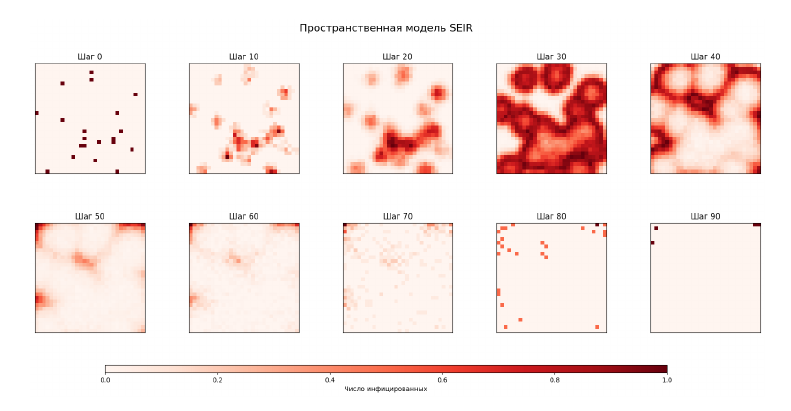
\includegraphics[scale=0.5]{../images/screenshot009}
		\caption{}
		\label{fig:screenshot009}
	\end{figure}
	
\end{frame}

\begin{frame}
	
	{Применение мультиагентной SEIR модели для моделирования}
	% TODO: \usepackage{graphicx} required
	\begin{figure}
		\centering
		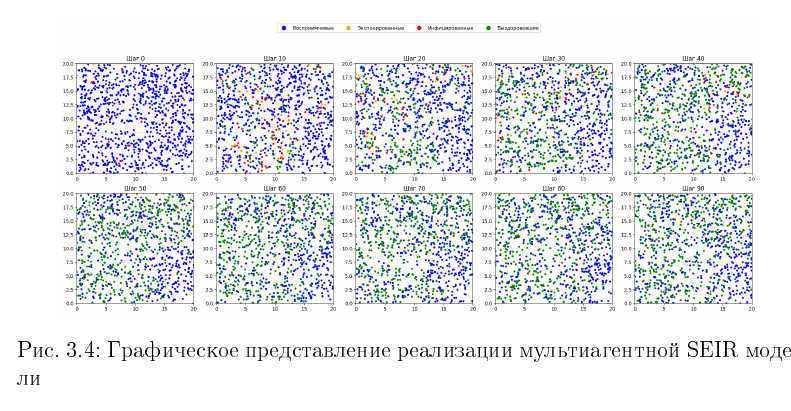
\includegraphics[scale=0.5]{../images/screenshot010}
		\caption{}
		\label{fig:screenshot010}
	\end{figure}
	
\end{frame}

\begin{frame}
	{Заключение}
	В данной работе рассмотрена SEIR-модель и ее расширения, с помощью которых был смоделирован процесс распространения заболеваний.
	В ходе работы
	\begin{enumerate}
		\item рассмотрена классическая SI-модель и ее аналитическое решение;
		\item рассмотрена классическая SIR-модель, вывод ее дифференциальных уравнений, исследование вопроса о корректной постановке задачи Коши, построение аналитического решения, описание методов построения приближенного решения;
		\item рассмотрены основные базовые модификации SIR-модели: SIS, SIRS, SIRD, SEIR, MSIR, MSEIR;
		\item рассмотрены расширения базовой SEIR модели: вероятностная модель, пространственная модель, мультиагентная модель;
		\item на практике были рассмотрены способы построения расширений для модели SEIR для решения задачи о моделировании распространения гриппа и приведены результаты моделирования.
	\end{enumerate}
\end{frame}

%--------------------------------------------------------------------------

\begin{frame}
	{Список используемых источников}
	\begin{enumerate}
		\item Statistical forecasting of the dynamics of epidemiological indicators for COVID-19 incidence in the Republic of Belarus / Yu. S. Kharin, V. A. Valoshka, O. V. Dernakova, V. I. Malugin, A. Yu. Kharin// Journal of the Belarusian State University. Mathematics and Informatics. - 2020. - № 3. - С. 36-50
		\item Methods of intellectual data analysis in COVID-19 research / O. V. Senko, A. V. Kuznetsova, E. M. Voronin, O. A. Kravtsova, L. R. Borisova, I. L. Kirilyuk, V. G. Akimkin// Journal of the Belarusian State University. Mathematics and Informatics. – 2022. – № 1. – С. 83-96
		\item Детерминированные и стохастические модели распространения инфекции и тестирование в изолированном контингенте/ Чигарев, А. В.,Журавков, М. А.,Чигарев, В. А.// Журнал Белорусского государственного университета. Математика. Информатика - 2021. - № 3. - С. 57-67
	\end{enumerate}
\end{frame}

%--------------------------------------------------------------------------

\end{document} 